%\documentclass[openany,a4paper,11pt]{kth-mag} % No blank pages
\documentclass[a4paper,11pt]{kth-mag}
\usepackage[swedish,english]{babel}
\usepackage{textcomp}
\usepackage{lmodern}
\usepackage{graphicx}	
\usepackage{modifications}
\usepackage{algorithmicx}
\usepackage{amsmath}
\usepackage{amssymb}
\usepackage{algpseudocode}
\usepackage{hyperref}

% Todo:
% Fix width of pictures. - Fixat
% Make a new roulette selection picture. - Fixed torsdag
% Check that all references are used. - Fixed torsdag
% Check that all figures are referred to. - Fixed torsdag
% Check that the bibliography is consistent. - Fixat
% Make sure hyphens are in all the correct places. See: http://oxforddictionaries.com/words/hyphen, e.g. decision-making
% Decision making - Fixed torsdag
% All "section" should use small S. - Fixed torsdag
% All "figure" should use large F. - Fixed torsdag
% Define brains - Fixat
% Upload code to github and refer in appendix b - Fixat 
% Sortera listan med k�llor i bokstavsordning - Fixat

\title{Evolution of Artificial Brains in Simulated Animal Behaviour}
\subtitle{Using radial basis, linear and random functions for decision-making}
\foreigntitle{Evolution av artificiella hj�rnor vid simulering av djurs beteende}
\author{Bj�rn Tegelund\\Johan Wikstr�m}
\date{April 2013}
\blurb{Bachelor's Thesis at CSC\\Supervisor: Petter �gren\\Examiner: M�rten Bj�rkman}
\trita{TRITA xxx yyyy-nn}
\begin{document}
\frontmatter
\pagestyle{empty}
\removepagenumbers
\maketitle
\selectlanguage{english}
\begin{abstract}
In this report we simulate artificial intelligence in animals using genetic algorithms. 
In similar models, advanced artificial neural networks have been used for decision making. 
We present two simpler decision-making models. 
Using two models based on linear and radial basis functions we find similar behaviours as those found in other studies, including food seeking, obstacle avoidance and predator-versus-prey dynamics.
 
The results show that both decision-making models are equally efficient at gathering food and avoiding obstacles. 
The models differed in survival strategies when faced with dangerous obstacles and in a predator-versus-prey situation the predators based on radial basis functions performed better. 

Some evolutionary phenomena were observed during the evolution of the animals, including an evolutionary arms-race between predator and prey. 
We hoped to find signs of mimicry as well, but classic mimicry was not found in the results.

\end{abstract}
\clearpage
\begin{foreignabstract}{swedish}
I denna rapport simulerar vi artificiell intelligens hos djur med hj�lp av genetiska algoritmer. 
I liknande modeller har man tidigare anv�nd avancerade artificiella neuronn�t som beslutsmodeller. 
I denna rapport presenterar vi tv� enklare beslutsmodeller. 
Med tv� modeller baserade p� linj�ra och radiella basfunktioner hittas liknande beteenden som i tidigare rapporter, inklusive f�doletande, hinderundvikande och predator-bytesdjursdynamik.

Resultaten visar att b�da beslutsmodeller �r lika effektiva vid f�doletande och hinderundvikande. 
Modellernas �verlevnadsstrategier skiljer sig n�r farliga hinder inf�rs och i predator-bytesdjurssitationer �r predatorn baserad p� radiella basfunktioner effektivare.

Vissa evolution�ra fenomen observerades under evolutionen av djuren, inklusive en evolution�r  kappl�pning mellan bytesdjur och predator. 
Vi hoppades �ven finna tecken p� mimikry, men klassisk mimikry observerades inte i resultaten.

\end{foreignabstract}
\clearpage
\tableofcontents*
\mainmatter
\pagestyle{newchap}
\chapter{Introduction}

\section{Background}

Today's environment is becoming more and more extreme.
This makes it increasingly important to model and simulate different ecological scenarios.
A typical scenario could be moving a species of animals from one ecosystem to another, or predicting which species may face extinction in a continuously changing environment.
What these scenarios have in common is that the animals need to adapt to the changes occurring around them. 
They need to evolve new traits and behaviours to survive.
An important tool used to model evolution is genetic algorithms, which simulate evolution to approximate an optimal solution to an algorithmic problem.

Genetic algorithms have been used on several occasions to simulate artificial life as well as artificial intelligence and this report is a continuation of that research, focusing on the behaviour of the animals.
They have for example been used for training machine learning algorithms \cite{montana}, for robot motion planning \cite{huijsmann} and for training artificial neural networks in the ecosystem simulator Gaia \cite{gracias}.
The animals simulated in Gaia showed several interesting behaviours, two prominent ones being searching for food and obstacle avoidance. 
The authors of that report acknowledged that many of the behaviours observed could be implemented using simple linear associations instead of advanced and computationally expensive neural networks \cite{gracias}.
The goal of this report is to find out if that is possible.

\section{Scope and Objectives}

This report focuses on evolving simulated animal behaviour using two kinds of simple mathematical functions capable of linear associations, namely linear and radial basis functions. 
As a baseline, a decision-making model which makes random decisions is also used.  
Each decision-making model takes genes as input, which are produced by the genetic algorithm.
Each model can be thought of as the "brain" of the simulated animal.
Statistics such as learning capabilities, choice of strategy and how well the animals are able to adapt to their surroundings are then analysed. 

In nature evolution is not a straight-forward process. 
Instead, many different evolutionary phenomena affect the course a species takes when evolving.
A secondary goal of this project is therefore to see which evolutionary phenomena can be observed when running the simulation and in particular how they may relate to the animals' behaviour.

In each experiment the animals are presented with different surroundings, which can contain food, predators and other objects.
The two primary decision-making models are compared and contrasted after each experiment has been run, with the random model included when necessary. 

\section{Problem Statement}

\begin{enumerate}
\item Is it possible to simulate evolution of animal behaviour using linear and radial basis functions in combination with a genetic algorithm?
\item Are there any significant differences between the two decision-making models?
\item Which, if any, evolutionary phenomena can be observed in the simulated animals?
\end{enumerate}

\chapter{Technical Overview}

\section{Evolutionary Concepts in Nature}
\subsection{Overview}
\label{evolutionary_overview}
This section provides a short overview of the evolutionary concepts in nature which are mentioned in this report. 
As every solution that the genetic algorithm proposes can be thought of as an individual in a population, many natural evolutionary phenomena can be observed in these individuals as well.

\emph{Adaptation} is when an individual is forced to adapt to its surroundings in order to survive. 
In nature adaptation occurs over generations and the need to adapt is the primary motivator behind evolution \cite[p.~8]{king}. 
The fitness of an individual depends to a great extent on how well-adapted it is to its surroundings. 
During extreme environmental change the adaptation is accelerated and once the population can survive the adaptation rate decreases.
A large population size increases the ability to adapt, as a large number of potentially helpful adaptations can be made per generation. 
A smaller population is more unstable and vulnerable as random environmental changes can eradicate important individuals or genes from the population. 
An example of adaptation in nature is how the polar bear evolved to have thicker, whiter fur when moving to a colder, snow-covered environment.

\emph{Co-evolution} is when the evolution of a species is affected by the evolution of another \cite[p.~90]{king}. 
This could be both in a symbiotic, parasitic or a predator-versus-prey manner. 
When in a predator-versus-prey situation and the predator evolves faster, the prey is usually faced with extinction. 
If it is the other way around the predators are faced with extinction as they may not be able to catch enough prey for their population to survive. 
An example of this is the evolutionary arms-race between the cheetah and its prey, which are in a constant battle of being able to run the fastest.

\emph{Mimicry} is a kind of adaptation where one species mimics an object's appearance or behaviour \cite[p.~278]{king}. 
This could be camouflaging oneself as a stone or evolving brightly coloured patterns, characteristic of poisonous animals, despite not being poisonous. 
Mimicry can be found in certain species of butterflies which wings take on the shape, colour, and texture of leaves.

\section{Genetic Algorithms}

\subsection{Overview}
\label{ga_overview}

Genetic algorithms are a way of approximating solutions to NP-hard problems, a group of problems that are computationally expensive. 
Genetic algorithms are a form of machine learning algorithm typically used to solve problems with a large or complex search space and where other machine learning algorithms fail \cite[p.~269-288]{marsland}. 
Genetic algorithms resembles evolution in nature by defining a set of genomes, or individuals, where each genome represents a possible solution to the given problem. 
This genome is commonly stored as a string of zeros and ones or as a list of floating point values. 
This set of genomes undergoes several iterations, or generations, of small improvements by fitness evaluation, selection, mutation and crossover. 
These operators all have equivalents in natural evolution and eventually the genomes will converge to a solution which represents a local minima in the search space. 
The advantage of genetic algorithms is that the crossover operator enables a wider search over the problem domain than many other approaches, using fewer calculations \cite{holland}. 
In the following subsections, the most crucial parts of the genetic algorithm will be explained and in Figure \ref{algorithm-overview}   an overview of the genetic algorithm in pseudo code is depicted.

\begin{figure}
\begin{algorithmic}
\State $ S \gets $ a random distribution of genes
    \While {the genes have not converged towards a solution}

        \State $F\gets fitness(S)$
		\Comment Calculate fitness values for all $s \in S$
		\State $X \gets select(S,F)$
		\Comment Get a multiset of S using fitness values
		\State $C \gets crossover(X)$
		\Comment Apply crossover operator on multiset
		\State $M \gets mutate(C)$
		\Comment Apply mutation operator on crossed genes
		\State $S \gets M$
		\Comment Restart with the new generation
    \EndWhile
\end{algorithmic}
\caption{An overview of the genetic algorithm used in the experiments.}
\label{algorithm-overview}
\end{figure}

\subsection{Fitness}
\label{ga_fitness}
Fitness is the only mean of measuring the success of a solution. 
In nature, fitness is determined by the number of offspring produced by an individual and the percentage of the offspring which survive long enough to generate new offspring\cite[p.~117]{darwin}. 
In 1932, Sewall Wright suggested that species adapt until they reach a local maxima in a fitness search space, which is a multidimensional space consisting of all possible combinations of genes and their resulting fitness. 
To reach another local maxima in the search space, which might be higher than the previous, the species must journey through a "valley" in the search space that would result in a temporarily lower fitness \cite{wright}. 
In genetic algorithms, the fitness value can be any numerical value that describes each individual's success at solving the problem at hand, determined by a fitness function. 
Genetic algorithms can get significant performance advantages by selecting the correct fitness function. 
The fitness function should be strictly positive for all inputs and preserve some form of relative internal ordering of the individuals. 
In most problems there are multiple choices of fitness functions and the best choice of fitness function is unique for every problem \cite[p.~272]{marsland}. 
It is possible to force the individuals to use certain strategies by rewarding or penalising an individual's fitness when showing certain behaviour, but that is not desired in this project.
In nature survival strategies vary and that is a property which should be reflected in the simulation. 
Therefore the life length of the individuals was chosen as the fitness function, so that the animals can choose survival strategy freely.

\subsection{Selection}
Selection is the process of selecting which organisms that should be allowed to reproduce and in what proportions. 
In nature selection is closely tied to fitness as the individual which displays highest fitness is selected to mate most often.
In genetic algorithms there are several different ways to model the selection process, but it should always be dependant on the fitness values of the population.
A good fitness function should therefore strike a balance between favouring the fittest individuals and allowing less fit individuals to survive in a reduced number.  
One trivial selection function could be to select all individuals that pass a certain fitness threshold \cite[p.~273]{marsland}. 
This is a bad idea, however, since there are few ways to determine the correct threshold value. 
In the beginning of the evolution, a high threshold will exclude most of the genomes due to low general fitness and this will lead to a fast reduction of genetic variation. 
In the later stages of the evolution all individuals will pass the threshold, rendering the selection function useless.

A better approach is the so-called roulette wheel selection where each individual is mapped to an area of what looks like a roulette wheel (see Figure \ref{roulettewheelpic}). 
A larger fitness value means a larger area on the roulette wheel and the selection function simply generates random values corresponding to values on this roulette wheel. 
In this way, the individuals are chosen based on a biased stochastic variable and there is room for individuals with high fitness to dominate and for individuals with low fitness to be included by chance. 

\begin{figure}
\centering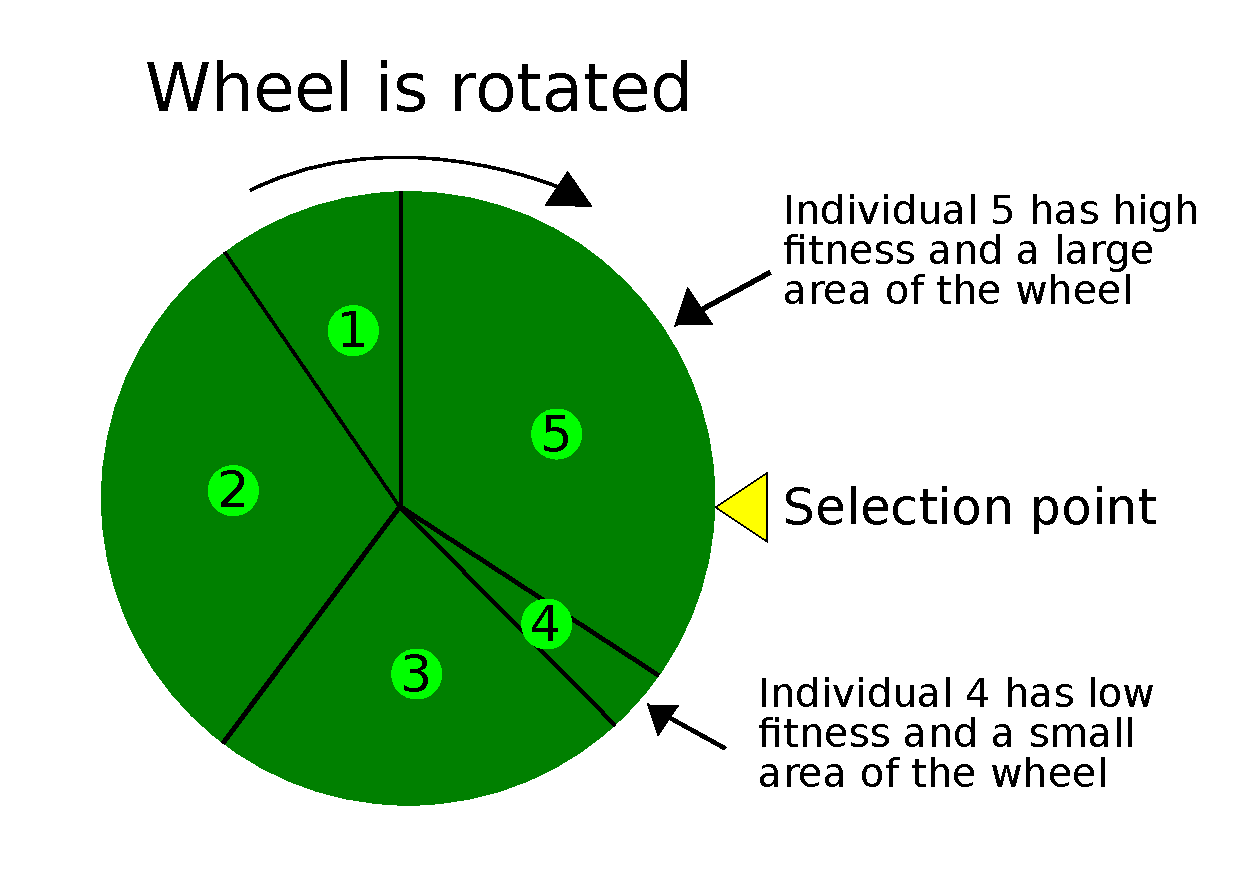
\includegraphics[height=0.35\textheight]{roulette.pdf}
\caption{A visual representation of how the roulette wheel selection algorithm works.}
% Beh�ver vi source till detta? Hittades h�r: http://www.edc.ncl.ac.uk/highlight/rhjanuary2007g02.php/
% G�r om denna!
\label{roulettewheelpic}
\end{figure}
 
\subsection{Mutation}
\label{background_mutation}
Mutation is a random, usually small, change in an individual's genome. 
In nature this typically occurs spontaneously when new cells are formed and there are hundreds of factors which can induce mutation \cite[p.~46]{vij} \cite[p.~289-290]{king}. 
In genetic algorithms it is usually implemented as a small probability for each gene to mutate. 
When the genome consists of a series of zero and ones, the mutation operator is a binary flip of that bit and when the genes consist of floating point values, the mutation can be an addition or multiplication of a random value. 
If the mutation rate is too high, it becomes hard to reach convergence since the good solutions will often be mutated into worse solutions.

\begin{figure}
\centering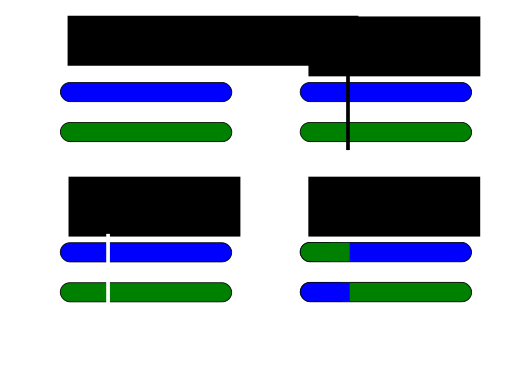
\includegraphics[scale=0.5]{crossover}
\caption{A schematic drawing showing single point crossover of two genomes.}
\label{crossover-figure}
\end{figure}

\subsection{Crossover}
Crossover is the operation of combining two genomes into two new genomes. 
One common crossover operator is known as  single point crossover and it consists of splitting two genomes at the same position and merging the split parts into two new genomes. 
The split position is chosen randomly and the two new genomes share no genes with each other. 
This process is displayed in Figure \ref{crossover-figure}. 
There is also multiple point crossover where there are multiple splitting positions as well as uniform crossover where each gene can be exchanged with a certain probability.

\section{Radial Basis Functions}
\subsection{Overview}
\label{rbf_background}

\begin{figure}
\centering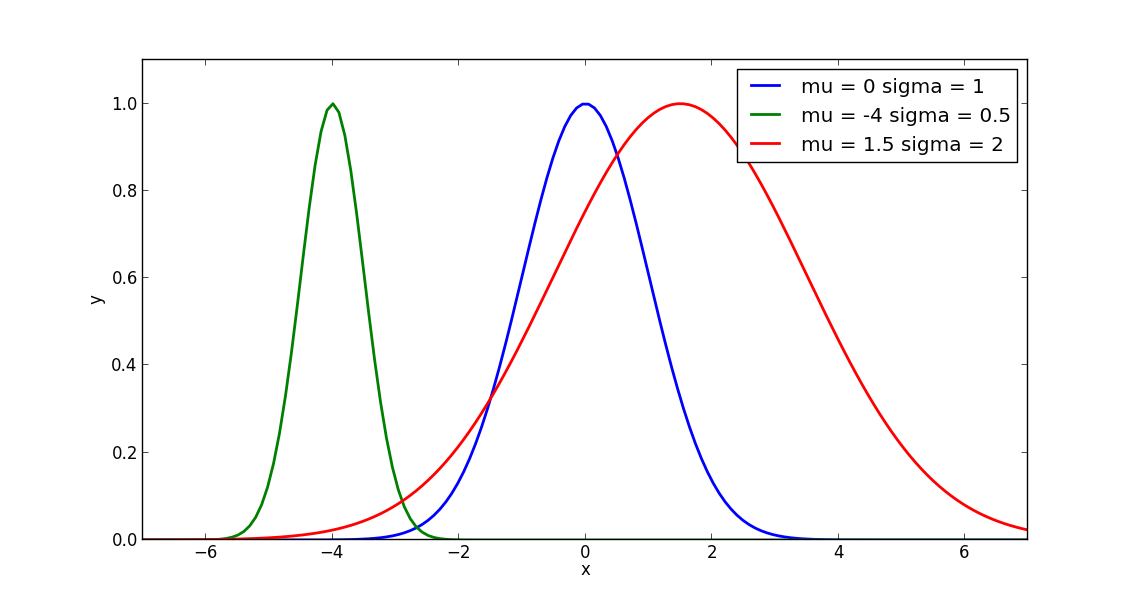
\includegraphics[scale=0.45]{rbf_1d.png}
\caption{Three one-dimensional RBFs with varying $\mu$ and $\sigma$ values. $\mu$ determines the centre of the bell curve and $\sigma$ controls the slope of it.}
\label{3-RBF-functions}
\end{figure}

A radial basis function (RBF) is a bell-shaped function whose value depends on the distance from some centre \cite[p.~1-8]{buhmann}, as shown in Figure~\ref{RBF-1}.
Radial basis functions are commonly used in artificial neural networks as a way to encode input information. 
They are favourable to use as they have locality, something which linear functions do not. 
Locality means that the function value is zero in almost the entire domain of the function. 
This is displayed in Figure~\ref{3-RBF-functions}. 
Locality makes them useful for function approximation, as any function can be approximated as the sum of a number of weighted radial basis functions. 
A property of radial basis functions which can both be interpreted as an advantage and a disadvantage is that their value never exceeds a given constant, compared to a linear function which can grow to infinitely high or low numbers.

Radial basis functions are commonly implemented using a formula such as in Figure~\ref{RBF-1}, which is a three-dimensional function centred around $(\mu _{x}$, $\mu _{y}$, $\mu _{z})$. 
The width of the bell-curve in each dimension is determined by $\sigma _{x}$, $\sigma _{y}$ and $\sigma _{z}$ respectively.

\begin{figure}
\begin{equation*}
f(x,y,z) = A_x*\exp(-\frac{(x-\mu_{x})^{2}}{2 \sigma _{x}^{2}}) + A_y*\exp(-\frac{(y-\mu_{y})^{2}}{2 \sigma _{y}^{2}}) + A_z*\exp(-\frac{(z-\mu_{z})^{2}}{2 \sigma _{z}^{2}})
\end{equation*}
\caption{A sum of three radial basis functions, corresponding to three input values. $A_x$, $A_y$ and $A_z$ lies within the interval $[-1,1]$ and ensures that $f(x,y,z)$ can be negative.}
\label{RBF-1}
\end{figure}

\chapter{Implementation}
\section{Model}
\subsection{Implementation in Python}
\label{simulation-in-python}
Python was chosen as implementation language since it is a high-level language suited for quickly building prototypes. 
It also has an abundance of third-party libraries which helps reduce implementation time significantly. 
A third-party library called DEAP (Distributed Evolutionary Algorithms in Python) was used for the genetic algorithm. 
DEAP proved to be flexible enough for the task as it allows the user to define their own selection, mutation and crossover algorithms as well as mixing them with the accompanying built-in algorithms. 
Pygame and Matplotlib were used for graphical rendering, Pygame for rendering the actual simulation and Matplotlib for producing graphs from the extracted data. 
To increase performance Pypy, Numpy and Python's built-in support for multiprocessing were used to decrease runtime significantly. 
For a comprehensive list of the tools used, please see Appendix \ref{list-of-third-party-tools}.

\subsection{Simulated World}
\label{simulated_world}
A world model for simulating the animals was created using Python together with the libraries mentioned in the previous section.
The world contains animals, which are spheres with two antennae protruding from their bodies at angles $\pi /6$ and $-\pi / 6$. 
There are two kinds of animals in the world: herbivores and predators. 
The herbivores' colours are decided by their genes. 
There may also be predators in the world that are similar to herbivores in appearance but always have a strong red colour. 
While herbivores eat green plants, which are green circles placed randomly within the world, predators eat herbivores.
Herbivores also have to avoid red plants, which are red circles. 
These represent "bad" or poisonous food. 
After a plant is eaten there is a small probability each moment that a new one will be placed into the world at a random location.
The maximum number of red and green plants possible in the world is fixed, and it becomes increasingly probable to spawn a new plant if there only are a few left. 
There are also walls around the border of the world which the animals cannot pass through. 
The walls are coloured blue in order for the herbivores to be able to make a clear distinction between walls, plants, predators and other herbivores. 
How the world is represented graphically can be see in Figure~\ref{sim_pic}.
Collision and detection, which are the only means of interaction between two objects, are governed by the following rules:

\begin{enumerate}
\item Interaction between two objects occur when they collide. A collision occurs when the distance between the centres of the two objects is smaller than the sum of their radii. Exactly what happens depends on the type of the objects.
\item Detection occurs when an object crosses the antennae of either a herbivore or predator.
\end{enumerate}

\begin{figure}
\centering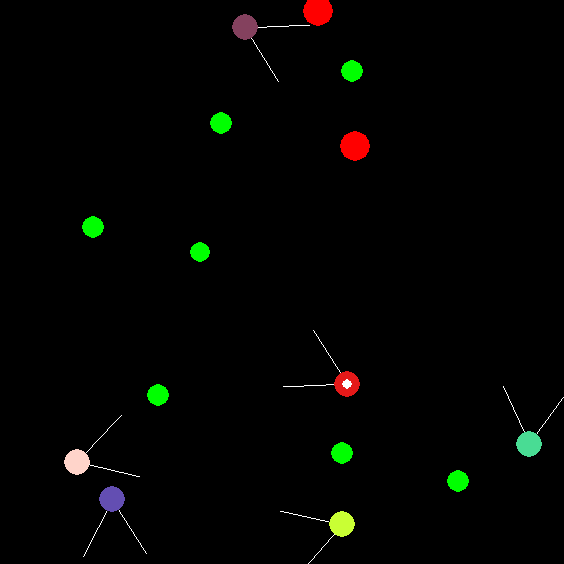
\includegraphics[scale=0.5]{simulation.png}
\caption{A screenshot of the simulation, showing green plants (green circles), red plants (slightly larger red circles), herbivores (multicoloured circles with antennae) and a predator (red circle with inner white circle and antennae).}
\label{sim_pic}
\end{figure}


At each moment, every possible collision is evaluated and the occurred collisions' effects are then applied immediately.
If a herbivore collides with a plant, that plant is eaten.
When eating a green plant the herbivore's lifespan is increased slightly and when eating a red plant the herbivore is killed.
Collisions between predators and plants do not have any consequences.
If a predator and a herbivore collide, the herbivore is killed and the predator's lifespan increased.
After that a check for detection occurs and the animals which have detected objects are allowed to process their inputs, using the decision-making models described in sections \ref{decision_making} to \ref{random_decision_making}, and apply a $\Delta s$ and a $\Delta r$ (change in speed and rotation) to their current speed and rotation. 
Every animal is then moved in accordance with their speeds and rotations. 

Due to performance issues, all animals of a population are not present in the same simulation. 
Instead, parts of the population are simulated separately. 
The results are then gathered and used to create the next generation. 
The detection and collision algorithms have a time-complexity of $O(n^{2})$ and therefore scale poorly. 
This the reason why the division of the population is needed. 
In practice this means that each simulation takes four times as long if the number of animals per simulation is doubled. 
By doing this trade-off with a lower number of animals in each simulation it was possible to run a higher number of iterations of the genetic algorithm in the same amount of time.

There are many specific constants which need to be fine-tuned for optimal results and performance, such as animal size,  speed and life length, among others. Listing all of these and their purposes would not contribute to this report, but the interested reader can find the entire source code for the project at the location specified in Appendix \ref{src_code}.

\subsection{Methods of Enforcing Behaviour}

In order to investigate the natural evolutionary phenomena that can be observed when using genetic algorithms, is it necessary to find methods of enforcing behaviour in the animals. 
It is also interesting to see which evolutionary strategies are favoured by the different brains when placed in particular situations. 
Methods of doing this could be either adding additional inputs to the brains or adding extra terms in the calculations to allow the approximation of more complex functions and thus more complex behaviour. 
This approach does however come at the cost of computing power. 
For each gene added the expected time for convergence is increased \cite{marsland}.

To focus more on which natural evolutionary phenomena occur, an approach was chosen which focused more on changing the animals' environment instead of the animals themselves. 
An example of an approach used was to add red plants into the world. 
The task of eating green plants then became more difficult as the animals also had to avoid mistakingly colliding with red plants. 
Another addition which allowed for more dynamics in the world was the choice to allow the herbivores to have different colours which also depended on their genes. 
By doing this it enabled the use of the evolutionary strategy known as mimicry, described in section \ref{evolutionary_overview}.

\subsection{Decision Making}
\label{decision_making}
All brains in our simulation have a similar structure, they are functions with eight inputs and two outputs. 
When input is received by an animal, it is in the form of eight numbers, four for each antenna. 
Three of the inputs for each antenna are the red, green, and blue components of the currently detected object's colour. 
These inputs are normalised to the interval $[0,1]$. 
The fourth input is zero when no object is detected and one when an object is. 
It was deemed necessary to include the fourth input to avoid certain edge-cases.
For example, if an animal were to detect a black object this would be equal to not detecting anything at all if using only three inputs, which in turn would give no reaction.

The outputs produced from this consists of the values $\Delta r$ and $\Delta s$ which denote changes in rotation and speed. 
Both output values are normalised to the interval $[-1,1]$ to account for the possibilities of negative rotation and negative acceleration. 
These values are then translated into reasonable values in the simulation. 
The maximum acceleration is determined by the size of the animals, the size of the world and the maximum speed of the animals.
This enables scaling of the world without affecting the simulation itself, by tweaking those constants. 
The maximum allowed change in rotation is 180$^\circ$ or $\pi$ since the interval $[-\pi,\pi]$ covers the entire circle. 
A larger allowed change in rotation would have made learning harder as there would be multiple correct responses to a situation, e.g $\Delta r = v, \Delta r = v+ 2\pi, \Delta r = v+ 4\pi$ and so on.

\subsection{Linear Decision Making}
\label{linear-decision-making}
The linear brain is a simple model for artificial intelligence. 
There are in total twelve genes associated with the brain in the interval $[-1,1]$.
These genes correspond to two outputs from the brain times two antennae times three colours.
Both $\Delta r$ and $\Delta s$ are calculated using the same method as mentioned in the previous section.

In Figure \ref{linear-decide}, the first three components of the left and right antennae vectors, the ones containing the colour data, are called $\mathbf{x_{l}}$ and $\mathbf{x_{r}}$ respectively. 
The fourth components are called $l_4$ and $r_4$, and show if an object has been detected or not, as mentioned earlier.
Six out of the twelve genes involved in total in the linear brain apply to this equation and they are divided into two vectors $\mathbf{g_{1-3}}$ and $\mathbf{g_{4-6}}$ using genes 1-3 and 4-6. 
The change in speed $\Delta s$ is calculated in the exact same way using the same inputs but genes 7-12 instead.

\begin{figure}
\begin{equation*}
\Delta r =
\begin{cases}
	0 																				& \text{if $l_4 = 0$ and $r_4 = 0$},\\
	S(\mathbf{g_{1-3}} \circ \mathbf{x_l}) 											& \text{if $l_4 \neq 0$ and $r_4 = 0$}\\
	S(\mathbf{g_{4-6}} \circ \mathbf{x_r}) 											& \text{if $r_4 \neq 0$ and $l_4 = 0$}\\
	S(\mathbf{g_{1-3}} \circ \mathbf{x_l} + \mathbf{g_{4-6}} \circ \mathbf{x_r} ) 	& \text{if $r_4 \neq 0$ and $l_4 \neq 0$}\\
\end{cases}	
\end{equation*}
\caption{The linear brain's decision formula for change of rotation $\Delta r$. $S$ corresponds to a sigmoid function described in section \ref{linear-decision-making}.}
\label{linear-decide}
\end{figure}

In Figure \ref{linear-decide} a sigmoid function $S$ is used to limit the outputs to be within $[-1,1]$. 
The function $\frac{1}{1+e^{-x}} * 2 -1$ was chosen as sigmoid function but any function $f:x\rightarrow y, x\in [-6,6], y \in [-1,1]$ would have worked as the only concern was to limit the output range to $[-1,1]$. 
The sigmoid function was however used as linear behaviour near $x=0$ was desired. 
That gives the best learning rate and a flatter curve at the extremes. 
An $x$ value near the extremes of $[-6,6]$ corresponds to radical behaviour such as turning 180$^\circ$ or accelerating rapidly and an $x$ value near 0 corresponds to making minor adjustments of speed and angle when encountering an object. 
A high $x$ value also corresponds to a rare event occurring, namely that both antennae detect objects with high colour values. 
As the objective was to train the animals to behave as rationally as possible to common events, the sigmoid function was chosen to slow down the learning rate of rare, extreme events and behaviours and accelerate the learning of common events and behaviours.
This corresponds to $x$-values in the sigmoid far from zero and near zero, respectively.
In this way, the animals still have the ability to make strong reactions, e.g. turning 180$^\circ$ when seeing a predator, but learning focuses more on the interesting behaviours, namely in which direction to turn or in which direction to accelerate. 
The reason for not choosing a simpler function, such as $f(x) = x/6$, as a normalising function was that it would have slowed down learning considerably giving more extreme cases a larger impact than desired.

\subsection{RBF-Based Decision Making}

In RBF-based decision making, the three inputs to each antenna are used in the function displayed in Figure~\ref{3-RBF-functions}. 
For each antenna, $\Delta r$  and $\Delta s$ are computed by summing radial basis functions' values and normalising them using the same function $S$ as in section~\ref{linear-decision-making}. 
As also mentioned in the same section, $\Delta r$ and $\Delta s$ are calculated separately using the same function and inputs but using different genes.

\begin{figure}
\begin{equation}
\Delta r =
\begin{cases}
	0 										&	\text{if $l_4 = 0$ and $r_4 = 0$},\\
	S(f(\mathbf{x_l})) 						&	\text{if $l_4 \neq 0$ and $r_4 = 0$}\\
	S(f(\mathbf{x_r})) 						&	\text{if $l_4 = 0$ and $r_4 \neq 0$}\\
	S(f(\mathbf{x_l}) + f(\mathbf{x_r})) 	&	\text{if $l_4 \neq 0$ and $r_4 \neq 0$}\\
\end{cases}	
\end{equation}
\caption{Calculating the $\Delta r$ using RBF functions. 18 genes are implicitly used, nine genes for $A$:s, $\sigma$:s and $\mu$:s in $f$ (see Figure~\ref{RBF-1}) using input $\mathbf{x_l}$ and nine for $\mathbf{x_r}$. }
\label{RBF-decide}
	\end{figure}

Each radial basis function has a $\sigma$ and a $\mu$ which are decided by the animals' genes. 
$\sigma$ and $\mu$ are in the ranges of $[0,1]$ and $[-1,1]$ respectively. 
An additional gene is also used to weight the output, which corresponds to $A$ in Figure~\ref{3-RBF-functions}. 
This is required to allow the otherwise positive radial basis functions to produce negative values as well. 
This means that the RBF-based brain has a total of 36 genes which need to be trained compared to the linear brain which only has twelve genes.

The difference between using radial basis functions and linear functions is that radial basis functions have a better ability to approximate any decision-making strategy, as mentioned in section~\ref{rbf_background}. 
For example, an RBF-based brain could make the distinction between different shades of green and thus react differently to them while a linear function could only decide if more green produces a stronger or weaker output.

\subsection{Random Decision Making}
\label{random_decision_making}
\begin{figure}
\begin{equation}
\Delta r = 
\begin{cases}
	0 		& 	\text{if $l_4 = 0$ and $r_4 = 0$},\\
	r \in U([-1,1])		&	\text{otherwise}
\end{cases}
\end{equation}
\caption{Calculating $\Delta r$ using random brain and the same notation as in Figure \ref{linear-decide} and Figure \ref{RBF-decide}. $r$ is a random number with uniform distribution.} 
\label{random-decide}
\end{figure}

In random decision making, only the fourth input which denotes whether an object has been detected or not, is used. If an object has been detected a $\Delta r$ and a $\Delta s$ within $[-1,1]$ are selected randomly with uniform probability. The sigmoid function $S$, which is used with both other brain architectures, is not used in the random brain, as the random values which are produced can easily be manipulated to be within the correct interval. 

\subsection{Genetic Algorithm}

The implemented genetic algorithm is similar to the one described in section~\ref{ga_overview}. 
The main difference is that a combination of selection methods are used. 
Instead of only applying roulette selection elitism is included as well. 
This means that 10\% of the next population are exact copies from the current generation's population, selecting the individuals with highest fitness. The modified algorithm is depicted in Figure~\ref{our_ga_overview}. 

Elitism is used as roulette selection is a highly probabilistic algorithm, and it is possible that some individuals with high fitnesses are not selected for the next generation. 
Elitism prevents these individuals from disappearing from the population by guaranteeing that their genes will survive until the next generation. 
Typically, these individuals also provide a stable maximum fitness for the population, as they are expected to perform equally well in the next simulation. 
It should however be noted that this is  not the case with the simulations discussed in this report, as both herbivore, plant, and predator placement are random.

Once individuals for the new generation have been selected, crossover and mutation are applied. The probability of applying crossover to a pair of individuals is 30\%. The probability of applying mutation is 40\%. Exactly what operators are used is described in the subsequent paragraphs in this section.

The crossover algorithm used for the experiments is a modified version of the uniform crossover algorithm mentioned in section~\ref{background_mutation}. 
If a uniform crossover algorithm is used, it could be the case that the $\mu$ of a radial basis function came from one parent and the $\sigma$ or $A$ from the other. 
This would most likely produce an individual with lower fitness than any of the its parents', as each parameter of a certain radial basis function has been tuned to be used together in the same calculation. 
Instead, "regions" of genes are replaced when applying crossover. 
A region is defined as a group of subsequent genes. 
For the RBF-based brains the size of these regions are three genes long while one gene long for the linear brains. 
This means that a radial basis function's $\mu$, $\sigma$ and $A$ are all copied. 
When crossover is applied, one calculation, i.e. a radial basis function or linear unit, for either speed or rotation and for either the left or right antenna is switched for the other parent's. 
The probability of exchanging the first individual's region for the second is 30\% for each region.

A gaussian mutator is chosen as mutation algorithm, as the animals' genes are floating point numbers. 
When mutation occurs a random number, distributed according to a gaussian distribution with mean $0$ and standard deviation $0.1$, is applied to the gene. 
On average, one gene is mutated per individual, as recommended in \cite{montana}.

\begin{figure}
\begin{algorithmic}
\State $S \gets$ a random distribution of genomes
\State $G \gets$ number of generations
    \For{$g \gets 1; g < G; g++$}
        \State $fitnesses \gets run\_simulations(S)$
	\Comment Simulates parts of $S$, collects result
	\State $couple\_fitnesses(S,fitnesses)$
	\Comment Associates a fitness value with an animal
	\State $B \gets select\_best(S, length(S)/10)$
	\Comment Select 10\% best genomes
	\State $R \gets select\_roulette(S, length(S) * 9/10)$
	\Comment Selects rest using roulette
	\For{$child1 \in R, child2 \in R$}
		\State $crossover(child1,child2)$
		\Comment Probabilistically applies crossover
	\EndFor
	\For{$child \in R$}
		\State $mutate(child)$
		\Comment Probabilistically mutates an individual
	\EndFor
	\State $S \gets B \cup R$
	\Comment Restart with the new generation
    \EndFor
\end{algorithmic}
\caption{An overview of the genetic algorithm used in the simulation.}
\label{our_ga_overview}
\end{figure}

\section{Experiments}
\subsection{Finding and eating food}
\label{exp1_desc}
This experiment consists of placing herbivores with randomly initialised genes in a world with only green plants in it. 
The number of green plants is variable, but never over a given maximum, and the results are checked after 300 generations. 
The population size is 200 and split into groups of 20 individuals, which are simulated separately. 
In each simulation the herbivores and plants are placed randomly into the world, with the herbivores having a random initial rotation. 
This is to avoid learning fixed patterns, that is doing the same sequence of actions each simulation. 
The downside of this is that the fitness values are not guaranteed to increase for each generation. Instead, a longer interval needs to be examined. 
As described in section~\ref{simulated_world}, a herbivore's life length is increased when eating a green plant and the fitness of a herbivore is its life length.

The purpose of this experiment is to see whether they are able to learn at all and how fast learning occurs. 
This will be an example of adaptation, as described in section~\ref{evolutionary_overview}, where the herbivores need to adapt to their new surroundings. 
It is also interesting to see if any specific behaviours occur in order to eat as many plants as possible. 
The results from the linear, RBF-based, and random brains are compared in order to see if there are any clear differences between them when running this initially simple experiment. 
It is expected that both types of brains are able to perform well in this task, as the problem is easy and solvable using colour associations, as proposed in \cite{gracias}.

In theory, a valid strategy could be to not react to plants at all. 
Simply accelerating to maximum speed and "combing" the world for plants by rotating randomly is a plausible strategy. According to \cite{gracias} a good strategy is to simply continue in the same direction and accelerate towards a plant when it is detected. 
Another strategy observed in the same paper was to follow the walls of the world.
Following the walls of the world can be a good strategy for poorly adapted individuals, since it provides an easy way to cover a large area and by chance encounter green plants.

\subsection{Avoiding bad food}
\label{exp2_desc}
This is a variation of the experiment described in the previous section, with the addition of red plants. 
Similar to the green plants, the number of red plants is zero at the beginning of the simulation and always below a fixed amount and they are also spawned in random locations. 
A problem with this approach is that a herbivore may be placed on top of a red plant, or vice versa. 
Nothing is done to prevent this, as with a large enough population size this is negligible. 
Another issue with this is that red and green plants could be placed above, or near, each other in the world, thus making it difficult for the herbivores to eat the green plant while avoiding the red plant. 
The expected result of this is a lower average fitness value, but it is allowed to happen in order to see how the different brain types react to this case.

By adding red plants to the simulation the task of living as long as possible becomes more complex. 
It is no longer a valid strategy to randomly pick a new direction each time a wall is encountered and not reacting to the detected plants. 
There are essentially two strategies for coping with this; the first strategy is trying to avoid red plants as much as possible, and the second is to focus more on eating green plants than avoiding red ones. 

\subsection{Predators and prey}
\label{exp3_desc}
In this experiment predators are added to the first and second experiment.
The ratio of predators to herbivores is one to ten, which means that for each group of 20 herbivores there will be 2 predators.
As mentioned in section~\ref{simulated_world}, the predators' objective is to eat herbivores and the predators have a strong red colour. 
This colour is used as prey are already learning to avoid red plants and if the predators are red as well it will be easier for them to avoid getting eaten. 
Because of the limitations of the linear brains, the RBF-based brains could have an unfair advantage if the predators could have multiple colours.
Due to the design of the world it is beneficial to be able to treat blue, green, and red objects differently, and if the colours are mixed it quickly becomes too difficult for the linear brains to handle, as their reactions are the sum of the reactions to the individual components of the colour.

In previous experiments there is no benefit in changing colour for the herbivores. 
In this experiment, however, it may be beneficial to try to mimic either predators or walls. 
When this phenomena occurs in nature it is known as mimicry and described in section~\ref{evolutionary_overview}. 
Another interesting evolutionary phenomena which could occur is co-evolution. 
In this simulation that could mean the predator's average fitness continuously increasing while the herbivores' fitness slowly decreases, or vice versa, if the herbivores become proficient at avoiding predators.

\chapter{Results}
\section{Simulation results}
\subsection{Finding and eating food}
\label{exp1_res}
After running the first experiment the conclusion can be drawn that the genetic algorithm is able to train the herbivores to eat plants. Compared to the random brain, they perform about 175\% better after training for 300 generations. 
Most of the increase in fitness did occur between generations 1 and 100, as seen in Figure~\ref{exp1_fitness}. 
The differences between the fitnesses of the linear and RBF-based brains are small, which could be attributed to the randomness in the experiments and the simplicity of the given task. 
As expected in section~\ref{exp1_desc}, there were mainly two prevalent food eating strategies during the experiments, namely following the walls of the world while looking for nearby food and the strategy of abruptly rotating in towards the centre of the world when encountering a wall. 
In all cases the herbivores accelerated and turned towards the green plants, which was also expected in section~\ref{exp1_desc} and mentioned in \cite{gracias}. 

\begin{figure}[htbp]
   \centering
   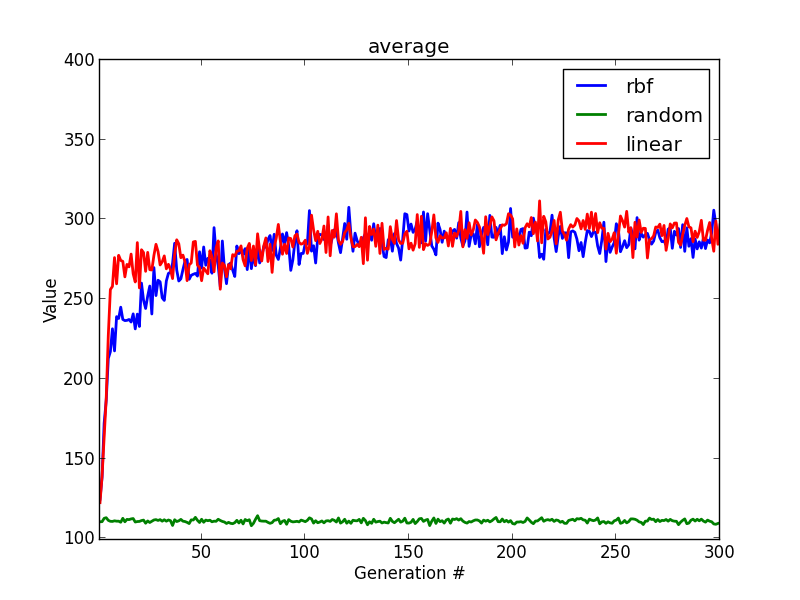
\includegraphics[height=0.45\textheight ,keepaspectratio]{exp1_fitness.png}
   \caption{A comparison between the average fitnesses of the RBF-based, linear and random brains when tasked only with eating green plants, according to section~\ref{exp1_desc}. It can be seen that the linear brains reach the fitness plateau faster.}
   \label{exp1_fitness}
\end{figure}

\begin{figure}[htbp]
   \centering
   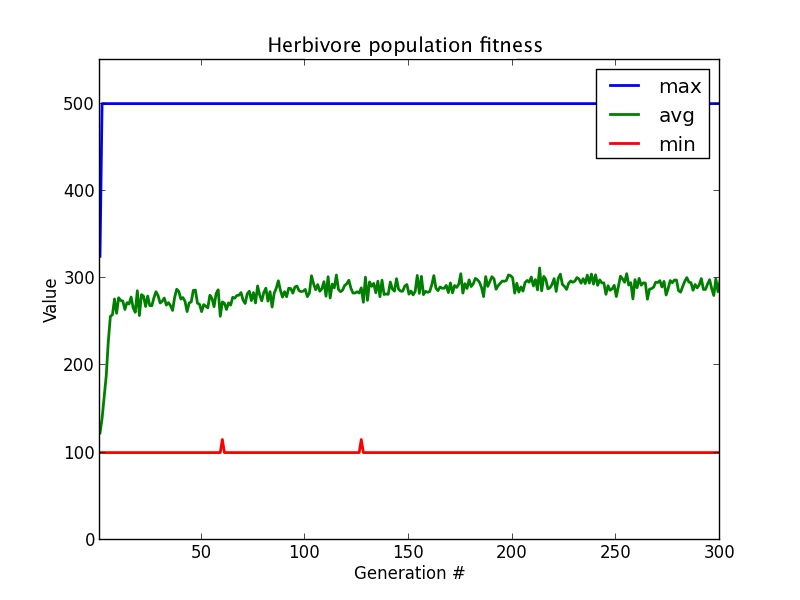
\includegraphics[height=0.45\textheight ,keepaspectratio]{exp1_linearfitness.png}
   \caption{A graph showing the minimum, average and maximum fitness per generation for a simulation using linear brains and only green plants, as described in section~\ref{exp1_desc}.}
   \label{exp1_linearfitness}
\end{figure}

The population size of 200 was found to be adequate as it provided a large enough genetic diversity within the population and was also small enough to be computationally cheap. 
High genetic diversity means a higher probability of initialising an individual with relatively successful genes, thus making the initial evolution faster. 
When using smaller population sizes the population and associated fitness values became more unstable and vulnerable to small random occurrences, such as a successful individual being randomly placed in a bad starting position. 
This can be related back to nature as an example of how smaller populations are unstable and more vulnerable, as stated in section~\ref{evolutionary_overview}.

The minimum and maximum fitness values for each generation were also of interest. 
As each individual is given a base life length of 100 the minimum fitness never went below 100. 
Due to the large population size and scarcity of plants in the world it was also seldom higher than 100.
There is almost always at least one unfit individual who will not eat a single plant for every generation. 
The maximum fitness reaches the maximum of a simulation after only a few generations, as shown in Figure \ref{exp1_linearfitness}. 
This means that one or several herbivores have survived the full length of the simulation.
It could be a problem if a large share of the herbivores reached the maximum, since these individuals would have the same fitness, but the average is low enough for this to not be a problem.
The average fitness increases steadily before reaching a plateau. 
The linear brains reached this plateau faster than the RBF-based brains, which could be an example of the longer convergence time for a higher number of genes.
This plateau represents a local maxima in the fitness search space, as mentioned in section~\ref{ga_fitness}. 
The likelihood of this local maxima being the global maxima is increased as both the linear and RBF-based brains reach the same maxima.  

The colours of the herbivores converged to a random point which reflects the decreasing genetic diversity within the population. 
All brains showed these tendencies in this experiment, which was expected, as there is no advantage or disadvantage associated with a certain colour.
An example of how the colours varied during the experiment can be found in Figure \ref{exp1_colour}.

\begin{figure}[htbp]
   \centering
   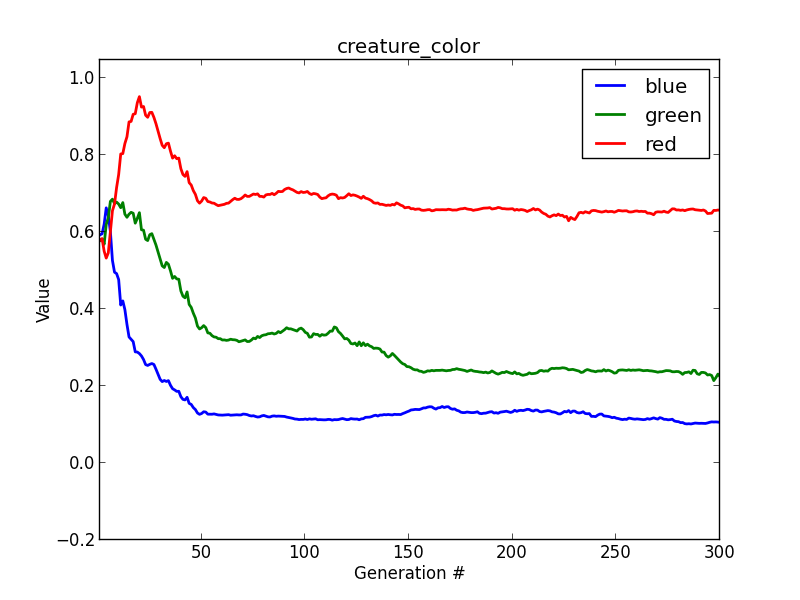
\includegraphics[height=0.45\textheight ,keepaspectratio]{exp1_colour.png}
   \caption{A graph over the change in the red, green, and blue components of the herbivores' colours during the experiment for the RBF-based brains with only green plants, according to section~\ref{exp1_desc}.}
   \label{exp1_colour}
\end{figure}

\subsection{Avoiding bad food}
Adding red plants to the simulation caused the fitness of both types of herbivores to decrease. 
When using a low maximum number of red plants no particular differences between RBF-based and linear brains were found. 
In both cases they managed to increase their fitness by about 100\% and approximately 40\% of all herbivores died from eating red plants. 
When doubling the amount of red plants in the simulation differences between the two decision-making models began to appear. 
Fitness was in both cases increased by about 30\%, but the ratio of herbivores killed from eating red plants differed, as shown in Figure \ref{exp2_deathrates}.
The linear brains had a death ratio between 60-70\% while the RBF-based brains had a ratio between 30-40\%.
This could indicate the use of different strategies. 
The linear brains seem to be more reckless by weighing the risk of eating a red plant against the possibility of eating many green plants. 
In comparison, the RBF-based brains seem to be more focused on avoiding red plants and being more cautious when approaching green plants.
A visual observation of the herbivores in action confirmed that few of the RBF-based herbivores ever collided with a red plant.
The differences in strategies is also supported by the fact that the maximum fitness for the linear brains is higher but also more unstable compared to the RBF-based brains.

In the previous experiment it was always beneficial to have the highest speed possible. 
In this experiment there were examples of herbivores moving slower than the maximum speed, particularly after detecting a red plant. 
This behaviour was found in both brains. 
One possible explanation of this could be that if they are traveling at maximum speed there is not enough time to successfully steer away from a red plant before colliding with it.
In this experiment the herbivores' colours converged to a random point, similar to the previous experiment.


\begin{figure}[htbp]
   \centering
   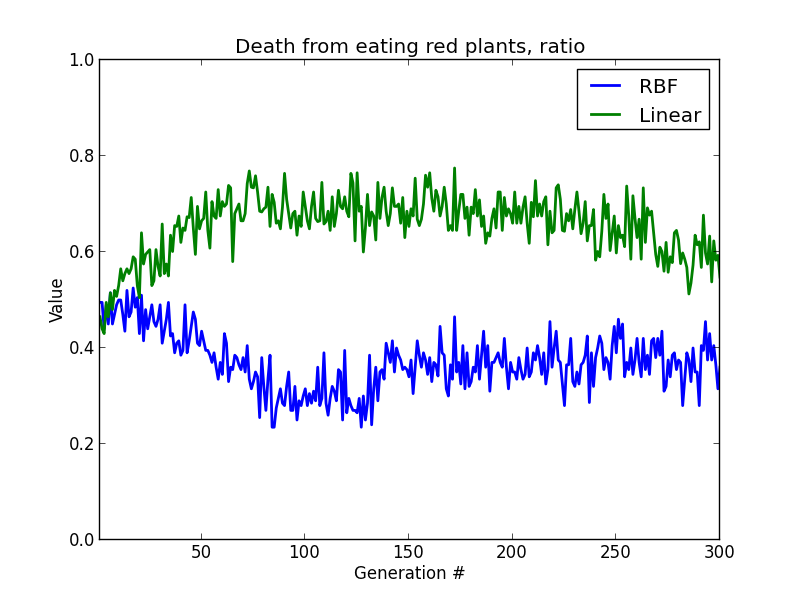
\includegraphics[height=0.45\textheight ,keepaspectratio]{exp2_deathrates.png}
   \caption{A graph showing the ratio of herbivores killed from eating red plants for both decision-making models. No predators were included in the experiment, as specified in section~\ref{exp2_desc}.}
   \label{exp2_deathrates}
\end{figure}

\subsection{Predators and prey}
In the simulation when only predators, herbivores and green plants were present the predators dominated. 
They achieved high fitness values and suppressed the herbivores' average fitness. 
Where in section~\ref{exp1_res}, with only herbivores and green plants, they had a fitness increase of about 175\% they were able to increase their fitness by 70-90\% at most for linear brains and 40-50\% at most for RBF-based brains. 

It was found that the herbivores with linear brains had both a higher death-rate by predators and higher fitness compared to RBF-based brains. 
Linear brains had a death rate of around 50\%, which was 10\% higher than the RBF-based brains, and a 90\% increase in fitness whereas RBF-based brains had a 30\% increase.
This indicates that RBF-based herbivores typically get eaten early on in the simulation, while linear herbivores survive longer before getting eaten.
RBF-based predators seem to be more effective than the linear predators, as they are able to eat a larger portion of their prey early on. 

In the linear case, signs of an evolutionary arms-race have been found where spontaneous changes in colours triggered a decrease in number of herbivores killed by predators, as shown in Figure \ref{exp3_lineardbp}. 
This suggests co-evolution between the herbivores and predators, as described in section \ref{evolutionary_overview}.
This in turn leads to the predators adapting to the herbivores' new colour, and again increasing the ratio of herbivores killed by predators. 
The arms-race was not as apparent with the RBF-based brains, which is believed to be due to the locality property of the radial basis functions. 
The locality property in this case means that a small change in colour can still give the same, or similar, reaction, which is believed to make them better predators as the herbivores' colours are dynamic during the initial phase of the simulation.
This is an example of where genetic algorithms do not perform well, as the vast majority of the RBF-based herbivores receive a low fitness value during the beginning of the simulation as they are eaten by predators and thus makes selection difficult.
It seems that difficulty when selecting which individuals are allowed to pass on their genes can give a decrease of the effectiveness of genetic algorithms. 
If a population of predators had had this kind of dominance over a population of prey in nature, the prey would likely be extinguished. 
However, due to the genetic algorithm the population survives and experiences the same scenario each generation.

\begin{figure}[htbp]
   \centering
   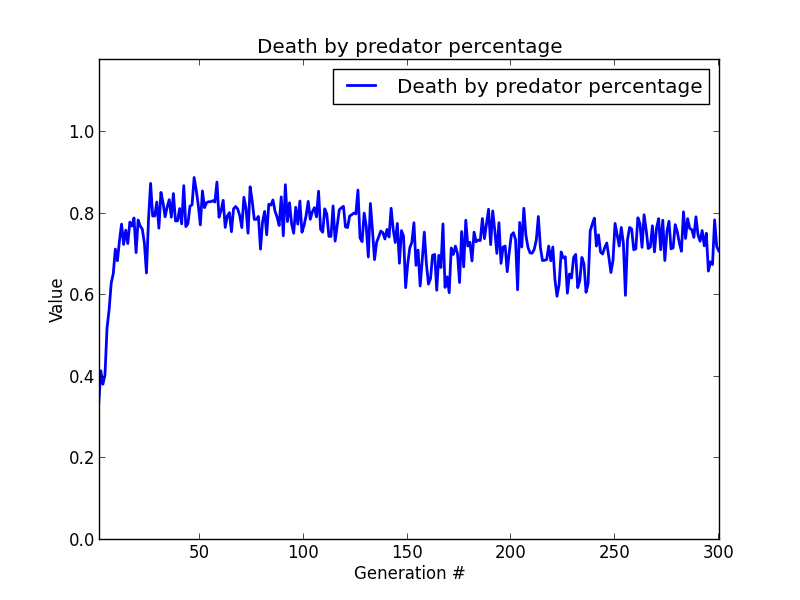
\includegraphics[height=0.45\textheight ,keepaspectratio]{exp3_lineardbp.png}
   \caption{A graph showing the herbivores' death-by-predator percentage when using linear brains, according to the specification in section~\ref{exp3_desc}. Decreases in the percentage correlate to sudden changes in the herbivores' colour.}
   \label{exp3_lineardbp}
\end{figure}

The colours in this experiment seemed to converge towards higher values, but without any clear strategy.
An example is shown in Figure \ref{exp3_rbfcolour}. 
It is believed that the strong colours which result from this are a way to fool the predators' brains into reacting strongly when detecting them. This reaction could be strong enough to send the predator in another direction, away from the herbivore. 
Initially it was believed that the herbivores would converge towards either a strong green, blue or red colour to mimic the objects already present in the world. 
An explanation as to why this did not occur could be that the motivation to increase one colour component while decreasing the two others is not apparent until perfect mimicry already has been reached.
When using Sewall Wright's analogy from section~\ref{ga_fitness}, the valley in the fitness landscape between the current peak and a peak where mimicry is present is too deep.

In the runs with both green and red plants it was observed that all animals had lower fitness. 
This was due to the herbivores dying of red plants which lead to predators having fewer herbivores to eat. 
In general, it seemed easier to avoid red plants than predators which is expected as the herbivores only can see in front of them. 
A clear inverse correlation was found between the ratio of herbivores killed by red plants and the ratio killed by predators. 
When herbivores learnt to avoid red plants they were instead eaten by predators and vice versa.
Apart from this no new results were found.

\begin{figure}[htbp]
   \centering
   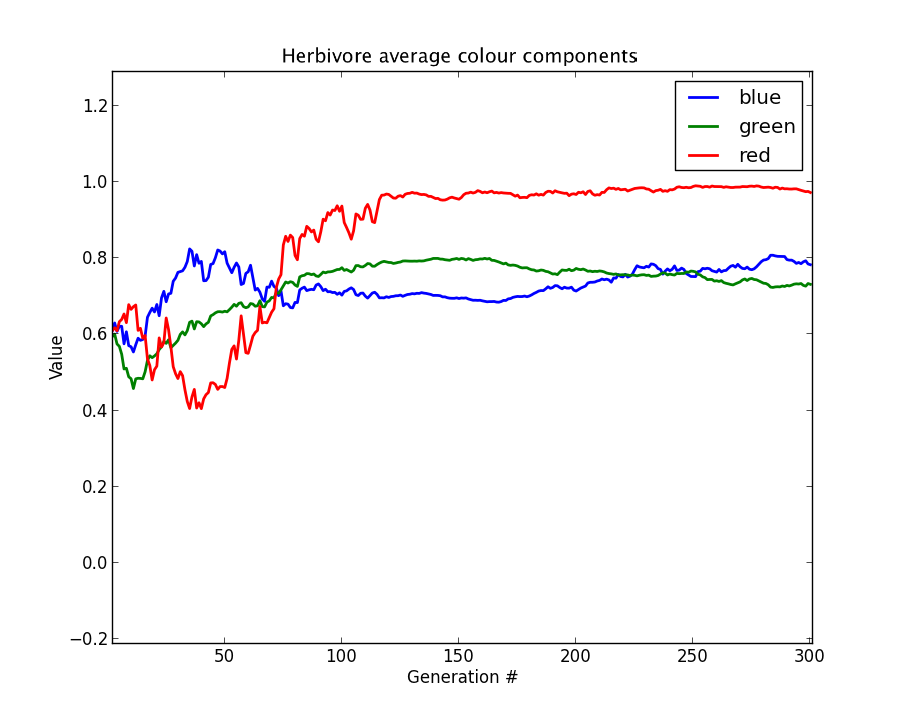
\includegraphics[height=0.45\textheight ,keepaspectratio]{exp3_rbfcolour.png}
   \caption{A graph over the change in the red, green, and blue components of the herbivores' colours during the experiment for the RBF-based brains with predators and green plants, according to section~\ref{exp3_desc}.}
   \label{exp3_rbfcolour}
\end{figure}

\section{Discussion}
\subsection{Constraints and Problems}
One serious and unexpected constraint was the performance of our algorithm. 
After profiling the code and making several improvements the performance was still a major issue. 
The main problem was the matching algorithms which compared all animals and plants to each other to determine collisions and detections. 
Checking all members of a list towards themselves is an operation which takes the time $O(n^2)$ on the size of the list and this is unacceptable as $n$ grows. 
The solution was to split up the population into several subpopulations, as mentioned in section~\ref{simulation-in-python}, and run their simulation separately, sequentially or in parallel. 
This trick reduces the time complexity to $O(K*n)$ where $K$ is a constant less than $n$.

The algorithms for collisions and detections were also scrutinised and all floating point calculations were replaced with pre-calculated values wherever possible. 
After the discovery of the scalar dot product as a big consumer of computation time, an alternative implementation was developed using pre-calculated values which sacrificed some memory and accuracy to achieve better running times. 
The standard Python implementation was also deemed too slow and PyPy, a fast Just-In-Time compiler was used to run the code most of the time. 
Finally, multiple cores were utilised by using Python's built-in support for multiprocessing. 
Python was chosen over C++ since Python allows for a much faster development process which made this project feasible given the allotted amount of time.

\subsection{Simulation Accuracy and Applications}

The model created in this project is mainly intended for studying evolutionary phenomena, not to provide a biologically accurate model of an ecosystem.
It is useful for modelling specific evolutionary scenarios, as the simple model reduces the amount of external parameters which may affect the simulation.
This could also have drawbacks as the model may be too simplified to realistically model real-life scenarios.
The most significant limitations of the model are:

\begin{itemize}
\item The antennae model is in most cases not a realistic input-gathering system. Each antenna can for example only detect one object at a time and the animals cannot control the antennae.
\item The predators have an unfair advantage as the herbivores cannot know if they are being chased.
\item The way reproduction works is simplified in the experiments. In real-life, reproduction is a continuous process and the population size is not fixed.
\item Due to the performance issues outlined in the previous section, the population sizes in each simulation are smaller than they would be in nature.
\end{itemize}

Despite these limitations the model was fully adequate to fulfil the goals of this project.
A more biologically correct model would not necessarily have helped answer the questions posed in this report better, since a less complex model using fewer parameters gives a clearer connection between cause and effect.
Using antennae to detect colours might not be biologically correct, but it still enabled the sought after behaviours to develop. 
Using colours also made analysis easier, as opposed to, for example, texture or shape, which may have been more biologically accurate. 
If another system for reproduction had been used it would have been more difficult to compare generations and the desired effects still appeared using the current system.

The simple deterministic brains used in the model could in some cases be a realistic model of real organisms. 
When considering primitive eucaryote and procaryote organisms, which employ limited movement and input capabilities, this model might still contain the complexity required to model their behaviour accurately.
It is however important to keep in mind that simulating growing populations is problematic due to the genetic algorithm used and performance issues.

\section{Conclusions and Future Work}
In this report it has been found that it is possible to simulate evolution of animal behaviour using both linear and radial basis functions. 
As theorised in \cite{gracias}, it is possible to model food-seeking strategies as well as more advanced survival strategies using linear associations. 
The food-seeking strategies observed in \cite{gracias}, namely following the walls of the world and accelerating towards food upon detection, were also developed by the animals simulated in this project.

The differences found between the when using radial basis functions and using linear functions were relatively small. 
When using linear functions the animals tended to use a more aggressive strategy when seeking food in a dangerous environment.
When encountered with both edible and poisonous food they chose a strategy where they risked eating poisonous food in return for eating a possibly larger portion of edible food.
The animals which used radial basis functions seemed to be more restrained, minimising the risk of eating poisonous food while losing some of the edible food.
Unexpectedly, both these strategies lead to similar performance of the animals' populations.
Another difference found was that the predators using radial basis functions were more successful in killing prey. 
It is however not certain that this applies in all situations, as more experiments are needed to fully investigate the reasons behind this.

Certain similarities between the model and natural evolution were observed. 
When the animals were first placed into the simulated world they behaved randomly and were not able to find and eat food.
The genetic algorithm incrementally improved their genes, thus making them adapt to their new environment well.
The animals had colours determined by their genes and when predators were introduced to the world the prey used this mechanism for self-defence.
It was expected that the prey would use mimicry to camouflage themselves as other objects within the world, but that was not the case.
Instead, a tendency to favour strong colours was found.
This could in many cases induce a stronger reaction in the predators, which could be to the predator's disadvantage.
This is an example of an evolutionary arms-race between the prey's ability to change their colour and the predator's ability to adapt to that change, which the prey in all cases lost during our simulations. 

This kind of simulation could be used in the future to examine other functions or strategies used for decision making as well. 
Even though mimicry was not clearly observed it is believed that it could be, given experiments specifically targeted towards it. 
It is also believed that this model could be modified to realistically model simple biological organisms, such as primitive prokaryotes or bacteria. 
The authors of this report hope that more similar projects will be done in future using genetic algorithms, as they tend to go beyond human imagination in search for potential solutions.

\begin{thebibliography}{99}

\bibitem{buhmann}
Buhmann, M. D. (2003) \emph{Radial Basis Functions: Theory and Implementations}. Cambridge University Press
\bibitem{darwin}
Darwin, C, (1861) \emph{On the origin of species by means of natural selection; or, The preservation of favoured races in the struggle for life}. D. Appleton and Company
\bibitem{gracias}
Gracias N., Pereira H., Lima J.A., Rosa A. (1997). Gaia: An Artificial Life Environment for Ecological Systems Simulation \emph{Artificial Life V: Proceedings of the Fifth International Workshop on the Synthesis and Simulation of Living Systems} 
\bibitem{holland}
Holland, J. H. (1992). Genetic algorithms. \emph{Scientific american, 267(1)} (pp. 66-72).
\bibitem{huijsmann}
Huijsmann, R., Haasdijk E., Eiben A. E. (2012) An On-line On-board Distributed Algorithm for Evolutionary Robotics. In \emph{Artificial Evolution} (pp. 73-84). Springer Berlin Heidelberg
\bibitem{king}
King, R. C., Stansfield W. D., Mulligan, P. K., (2006) \emph{A Dictionary of Genetics}. Oxford University Press
\bibitem{marsland}
Marsland, S. (2009). \emph{Machine Learning, an Algorithmic Perspective}. CSC-Press
\bibitem{montana} 
Montana, D. J.,  and Davis, L. (1989, August). Training feedforward neural networks using genetic algorithms. In \emph{Proceedings of the eleventh international joint conference on artificial Intelligence} (Vol. 1, pp. 762-767).
(Vol. 5). Mit Press.
\bibitem{vij}
Vij, K. and Biswas, R. (2004) \emph{Basics of DNA \& Evidentiary Issues}. Jaypee Brothers Publishers
\bibitem{wright}
Wright, S., (1932), The Roles of Mutation, Inbreeding, Crossbreeding and Selection in Evolution. In \emph{Proceedings of the Sixth International Congress on Genetics} (pp. 355-366). Brooklyn Botanic Garden
\end{thebibliography}

\pagestyle{plain}
\removepagenumbers
\listoffigures
\emph{Note:} all of the figures have been created by the authors.

\appendix
\addappheadtotoc
\chapter{Third-party libraries and tools used}
\label{list-of-third-party-tools}
\begin{itemize}
\item DEAP - Distributed Evolutionary Algorithms in Python \url{http://deap.gel.ulaval.ca/doc/default/index.html}
\item PyPy - A fast Just-in-Time compiler for Python. \url{http://pypy.org/}
\item Pygame - A computer game and visualisation package for python. \url{http://www.pygame.org/docs/}
\item NumPy - A Python package for numerical calculations. \url{http://www.numpy.org/}
\item matplotlib - A Python package for rendering graphs. \url{http://matplotlib.org/}
\end{itemize}

\chapter{Source Code}
\label{src_code}
The source code used to generate all of the results can be found at:\\
\url{https://github.com/johanwikstrm/artificialbrains}

\chapter{Statement of Collaboration}
Both authors have spent an equal amount of time working on and contributing to the code, experiments and this report.

\end{document}
